\documentclass{article}
\usepackage{tikz}
\usetikzlibrary{positioning} %on grid
\usetikzlibrary{automata} %style
\usetikzlibrary{shapes,snakes}%各中形状




\usepackage{wrapfig} %文字环绕
\usepackage{fontspec}



\begin{document}
We are working on
\begin{tikzpicture}
	\draw (-1.5, 0) -- (1.5,0);%-- 直线
	\draw (0,-1.5) .. controls (3,3) ..  (0,1.5); %..曲线
\end{tikzpicture}
\newline
\tikz \draw (-1.5,0) -- (1.5, 0) -- (0,-1.5) -- (0,1.5);
\newline
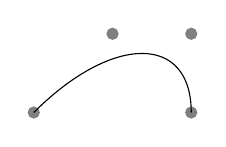
\begin{tikzpicture}
  \filldraw [gray] (0,0) circle (2pt)
                   (1,1) circle (2pt) %园 半径
                   (2,1) circle (2pt)
                   (2,0) circle (2pt);
  \draw (0,0) .. controls (1,1) and (2,1) .. (2,0);%controls xxx 作为曲线的控制点 
\end{tikzpicture}
\newline
\tikz \draw[rotate=30] (0,0) ellipse (20pt and 10pt); %椭圆, rotate参数控制旋转(逆时针,同极坐标)
\tikz \draw (0,0) rectangle (1, 1);

\tikz \draw[step=10pt, yellow, very thin] (0,0) grid (100pt, 100pt);%step步长, 参数长宽

\tikz \draw (0,0) arc (0:45:50pt); %弧, 50半径圆45度弧长
\tikz \draw (0,0) arc (0:315:50pt and 100pt);%弧, 长轴50短轴100 300度椭圆弧
\newline
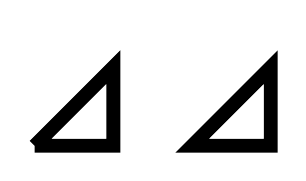
\begin{tikzpicture}[line width=5pt]
  \draw (0,0) -- (1,0) -- (1,1) -- (0,0);
  \draw (2,0) -- (3,0) -- (3,1) -- cycle;
  \useasboundingbox (0,1.5); %  make bounding box higher
\end{tikzpicture}

\tikz[>=stealth] \draw [->] (0,0) -- (5,5); %使用箭头,>=stealth指定样式

%使用坐标便宜话双线
\tikz \draw (0,0) -- (0,0.5) [xshift=2pt] (0,0) -- (0,0.5);

\foreach \x in {1,2,3} {$x =\x$}



%使用node
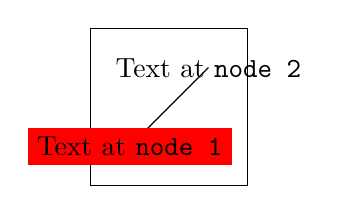
\begin{tikzpicture}
  \draw (0,0) rectangle (2,2);
  \draw (0.5,0.5) node [fill=red]
                       {Text at \verb!node 1!} -- (1.5,1.5) node {Text at \verb!node 2!};
\end{tikzpicture}

\tikzset{ state/.style={circle,draw=black,very thick}}
\tikzset{ term/.style={circle,very thick,double,draw=black}}

\begin{tikzpicture}[shorten >= 1pt, node distance=2cm, on grid, >=stealth]
\node[state]	(q_0)		{$q_0$};
\node[state]	(q_1) [above right=of q_0]	{$q_1$};
\node[term]	(q_2) [below right=of q_0]	{$q_2$};
\path[->]	(q_0)		edge				node	[above left]	{0}	(q_1)
				edge				node	[below left]	{1}	(q_2)
		(q_1)		edge	[loop above]	node				{0}	()
		(q_2)		edge	[loop below]	node				{1}	();
\end{tikzpicture}

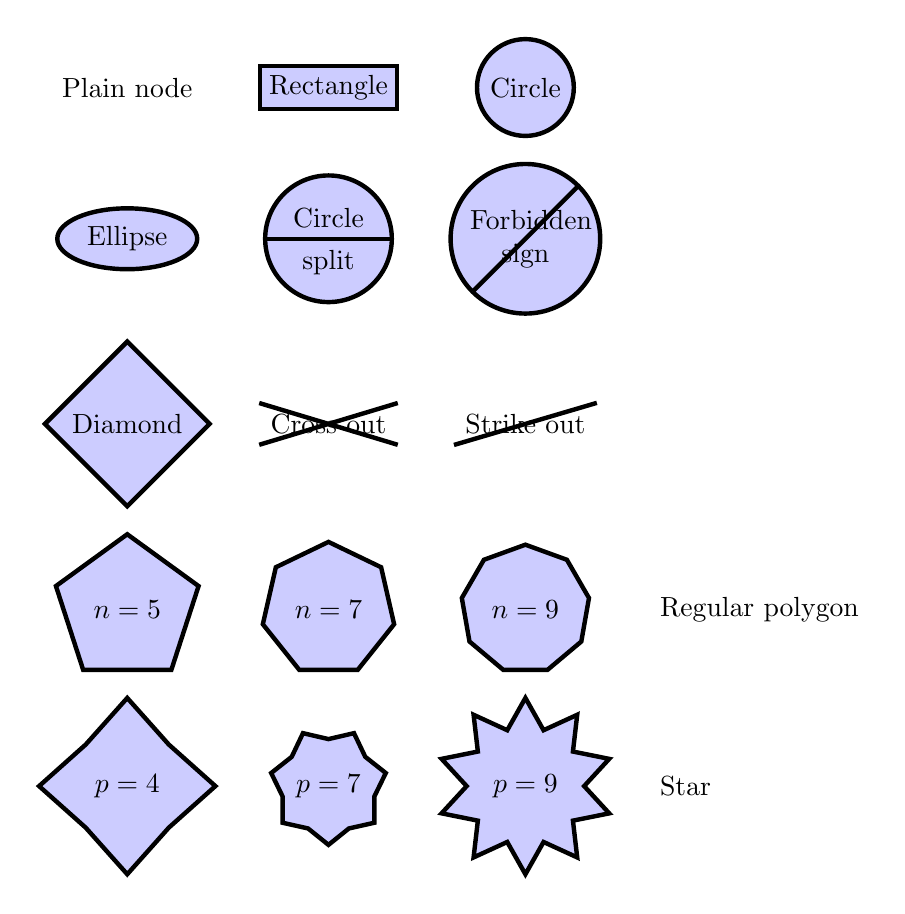
\begin{tikzpicture}[scale=2]
    \tikzstyle{ann} = [draw=none,fill=none,right]
    \matrix[nodes={draw, ultra thick, fill=blue!20},
        row sep=0.3cm,column sep=0.5cm] {
    \node[draw=none,fill=none] {Plain node}; &
    \node[rectangle] {Rectangle}; &
    \node[circle] {Circle};\\
   \node[ellipse] {Ellipse};&
    \node[circle split] {Circle \nodepart{lower} split};&
    \node[forbidden sign,text width=4em, text centered]
                    {Forbidden sign};\\
    \node[diamond] {Diamond};&
    \node[cross out] {Cross out};&
    \node[strike out] {Strike out};\\
    \node[regular polygon,regular polygon sides=5] {$n=5$};&
    \node[regular polygon,regular polygon sides=7] {$n=7$};&
    \node[regular polygon,regular polygon sides=9] {$n=9$};&
    \node[ann]{Regular polygon};\\
    \node[star,star points=4] {$p=4$};&
    \node[star,star points=7,star point ratio=0.8] {$p=7$};&
    \node[star,star points=10] {$p=9$};&
    \node[ann]{Star};\\
    };
\end{tikzpicture}

\end{document}
